\documentclass{standalone}

\usepackage{tikz}

\usetikzlibrary{calc}

\newcommand{\neuron}[3]{
    \node[circle, draw=black, fill=#2] (#1) at #3 {};
}

\begin{document}
    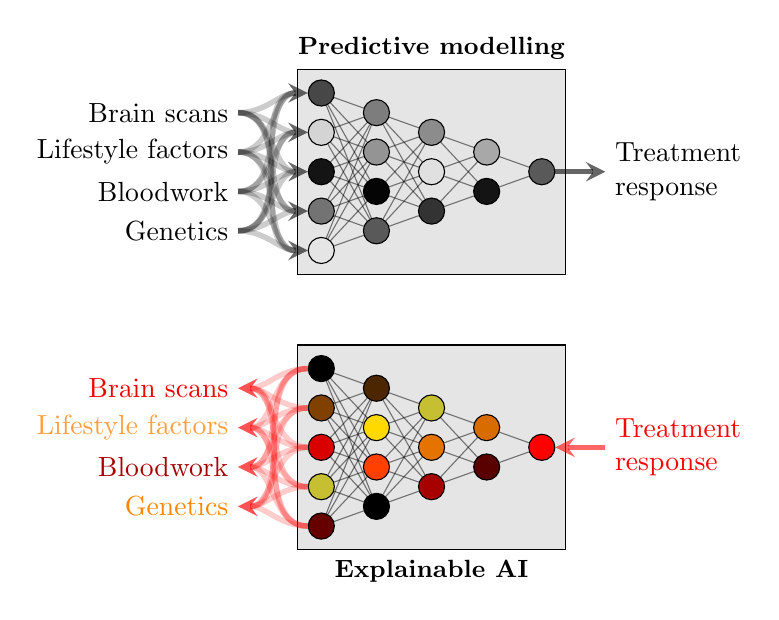
\begin{tikzpicture}
        \node[
            draw=black,
            fill=gray!20,
            minimum height=2.6cm,
            minimum width=3.4cm
        ] (model) at (0, 1) {};

        \node[anchor=south, font=\small\bfseries] at (model.north) {Predictive modelling};

        \def\hsep{0.7}
        \def\vsep{0.5}
        \def\edgecolor{gray}
        \def\edgeopacity{0.5}

        \node[anchor=east] (x0) at ($ (model.west) + (-0.75, 0.75) $) {Brain scans};
        \node[anchor=east] (x1) at ($ (model.west) + (-0.75, 0.25) $) {Lifestyle factors};
        \node[anchor=east] (x2) at ($ (model.west) + (-0.75, -0.25) $) {Bloodwork};
        \node[anchor=east] (x3) at ($ (model.west) + (-0.75, -0.75) $) {Genetics};

        \neuron{n00}{black!10}{($ (model) + (-2 * \hsep, -2 * \vsep) $)}
        \neuron{n01}{black!55}{($ (model) + (-2 * \hsep, -\vsep) $)}
        \neuron{n02}{black!92}{($ (model) + (-2 * \hsep, 0) $)}
        \neuron{n03}{black!17}{($ (model) + (-2 * \hsep, \vsep) $)}
        \neuron{n04}{black!72}{($ (model) + (-2 * \hsep, 2 * \vsep) $)}

        \neuron{n10}{black!65}{($ (model) + (-\hsep, -1.5 * \vsep) $)}
        \neuron{n11}{black!98}{($ (model) + (-\hsep, -0.5 * \vsep) $)}
        \neuron{n12}{black!42}{($ (model) + (-\hsep, 0.5 * \vsep) $)}
        \neuron{n13}{black!51}{($ (model) + (-\hsep, 1.5 * \vsep) $)}

        \neuron{n20}{black!80}{($ (model) + (0, -\vsep) $)}
        \neuron{n21}{black!12}{(model)}
        \neuron{n22}{black!45}{($ (model) + (0, \vsep) $)}

        \neuron{n30}{black!92}{($ (model) + (\hsep, -0.5 * \vsep) $)}
        \neuron{n31}{black!34}{($ (model) + (\hsep, 0.5 * \vsep) $)}

        \neuron{n40}{black!65}{($ (model) + (2 * \hsep, 0) $)}

        \node[anchor=west, align=left] (y) at ($ (model.east) + (0.5, 0) $) {Treatment\\response};

        \foreach \i in {0,...,4} {
            \foreach \j in {0,...,3} {
                \draw[-, black, opacity=\edgeopacity] (n0\i) -- (n1\j);
            }
            \foreach \j in {0,...,3} {
                \draw[-stealth, opacity=0.2, line width=2pt] (x\j.east) to [out=0, in=180] (n0\i);
            }
        }
        \foreach \i in {0,...,3} {
            \foreach \j in {0,...,2} {
                \draw[-, opacity=\edgeopacity] (n1\i) -- (n2\j);
            }
        }
        \foreach \i in {0,...,2} {
            \foreach \j in {0,...,1} {
                \draw[-, opacity=\edgeopacity] (n2\i) -- (n3\j);
            }
        }
        \foreach \i in {0,...,1} {
            \draw[-, opacity=\edgeopacity] (n3\i) -- (n40);
        }

        \draw[-stealth, opacity=0.6, line width=2pt] (n40) -- (y);

        \node[
            draw=black,
            fill=gray!20,
            minimum height=2.6cm,
            minimum width=3.4cm
        ] (model) at (0, -2.5) {};

        \node[anchor=north, font=\small\bfseries] at (model.south) {Explainable AI};

        \node[anchor=east, red!95!black] (x0) at ($ (model.west) + (-0.75, 0.75) $) {Brain scans};
        \node[anchor=east, orange!75] (x1) at ($ (model.west) + (-0.75, 0.25) $) {Lifestyle factors};
        \node[anchor=east, red!65!black] (x2) at ($ (model.west) + (-0.75, -0.25) $) {Bloodwork};
        \node[anchor=east, orange!95!yellow] (x3) at ($ (model.west) + (-0.75, -0.75) $) {Genetics};

        \neuron{n00}{red!40!black}{($ (model) + (-2 * \hsep, -2 * \vsep) $)}
        \neuron{n01}{yellow!75!black}{($ (model) + (-2 * \hsep, -\vsep) $)}
        \neuron{n02}{red!85!black}{($ (model) + (-2 * \hsep, 0) $)}
        \neuron{n03}{orange!50!black}{($ (model) + (-2 * \hsep, \vsep) $)}
        \neuron{n04}{black}{($ (model) + (-2 * \hsep, 2 * \vsep) $)}

        \neuron{n10}{black}{($ (model) + (-\hsep, -1.5 * \vsep) $)}
        \neuron{n11}{red!75!yellow}{($ (model) + (-\hsep, -0.5 * \vsep) $)}
        \neuron{n12}{red!15!yellow}{($ (model) + (-\hsep, 0.5 * \vsep) $)}
        \neuron{n13}{orange!30!black}{($ (model) + (-\hsep, 1.5 * \vsep) $)}

        \neuron{n20}{red!65!black}{($ (model) + (0, -\vsep) $)}
        \neuron{n21}{orange!90!black}{(model)}
        \neuron{n22}{yellow!75!black}{($ (model) + (0, \vsep) $)}

        \neuron{n30}{black!65!red}{($ (model) + (\hsep, -0.5 * \vsep) $)}
        \neuron{n31}{orange!85!black}{($ (model) + (\hsep, 0.5 * \vsep) $)}

        \neuron{n40}{red}{($ (model) + (2 * \hsep, 0) $)}

        \node[anchor=west, align=left, red] (y) at ($ (model.east) + (0.5, 0) $) {Treatment\\response};

        \foreach \i in {0,...,4} {
            \foreach \j in {0,...,3} {
                \draw[-, black, opacity=\edgeopacity] (n0\i) -- (n1\j);
            }
            \foreach \j in {0,...,3} {
                \draw[stealth-, opacity=0.2, line width=2pt, red] (x\j.east) to [out=0, in=180] (n0\i);
            }
        }
        \foreach \i in {0,...,3} {
            \foreach \j in {0,...,2} {
                \draw[-, opacity=\edgeopacity] (n1\i) -- (n2\j);
            }
        }
        \foreach \i in {0,...,2} {
            \foreach \j in {0,...,1} {
                \draw[-, opacity=\edgeopacity] (n2\i) -- (n3\j);
            }
        }
        \foreach \i in {0,...,1} {
            \draw[-, opacity=\edgeopacity] (n3\i) -- (n40);
        }

        \draw[stealth-, opacity=0.6, line width=2pt, red] (n40) -- (y);
    \end{tikzpicture}
\end{document}
